

\begin{figure}[H]
\centering
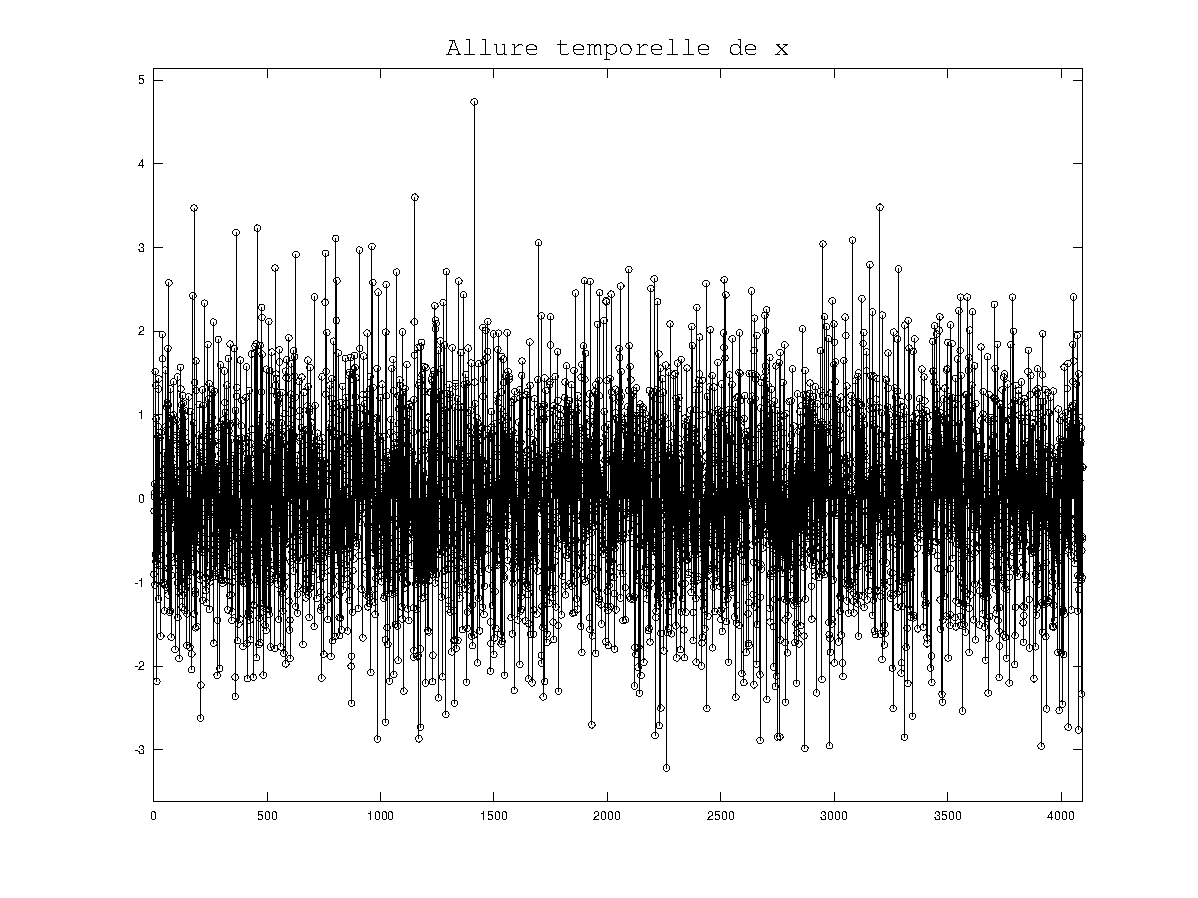
\includegraphics[width=9cm]{resEx6/fig_1.pdf}
\caption{Allure temporelle de x}
\end{figure}


\begin{figure}[H]
\centering
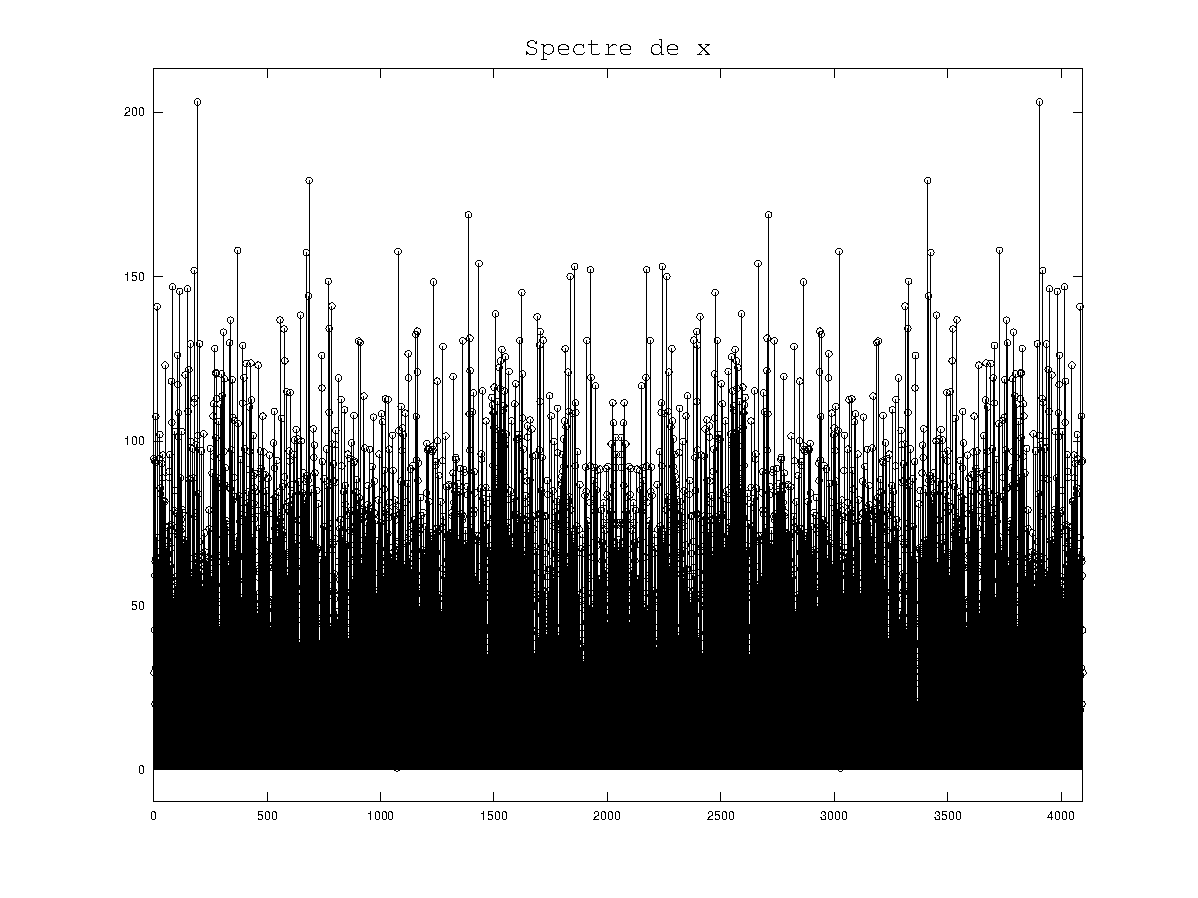
\includegraphics[width=9cm]{resEx6/fig_2.pdf}
\caption{Spectre de x}
\end{figure}


\begin{figure}[H]
\centering
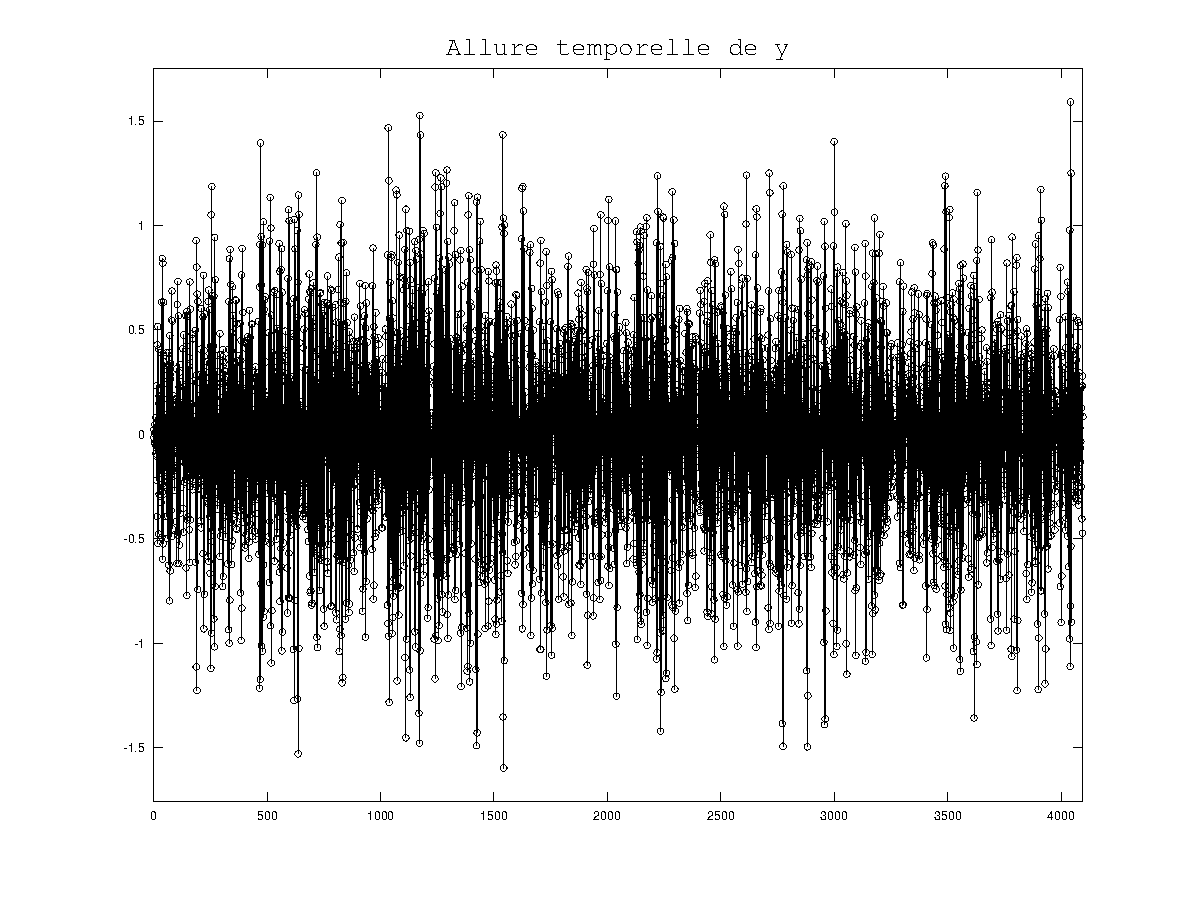
\includegraphics[width=9cm]{resEx6/fig_3.pdf}
\caption{Allure temporelle de y}
\end{figure}


\begin{figure}[H]
\centering
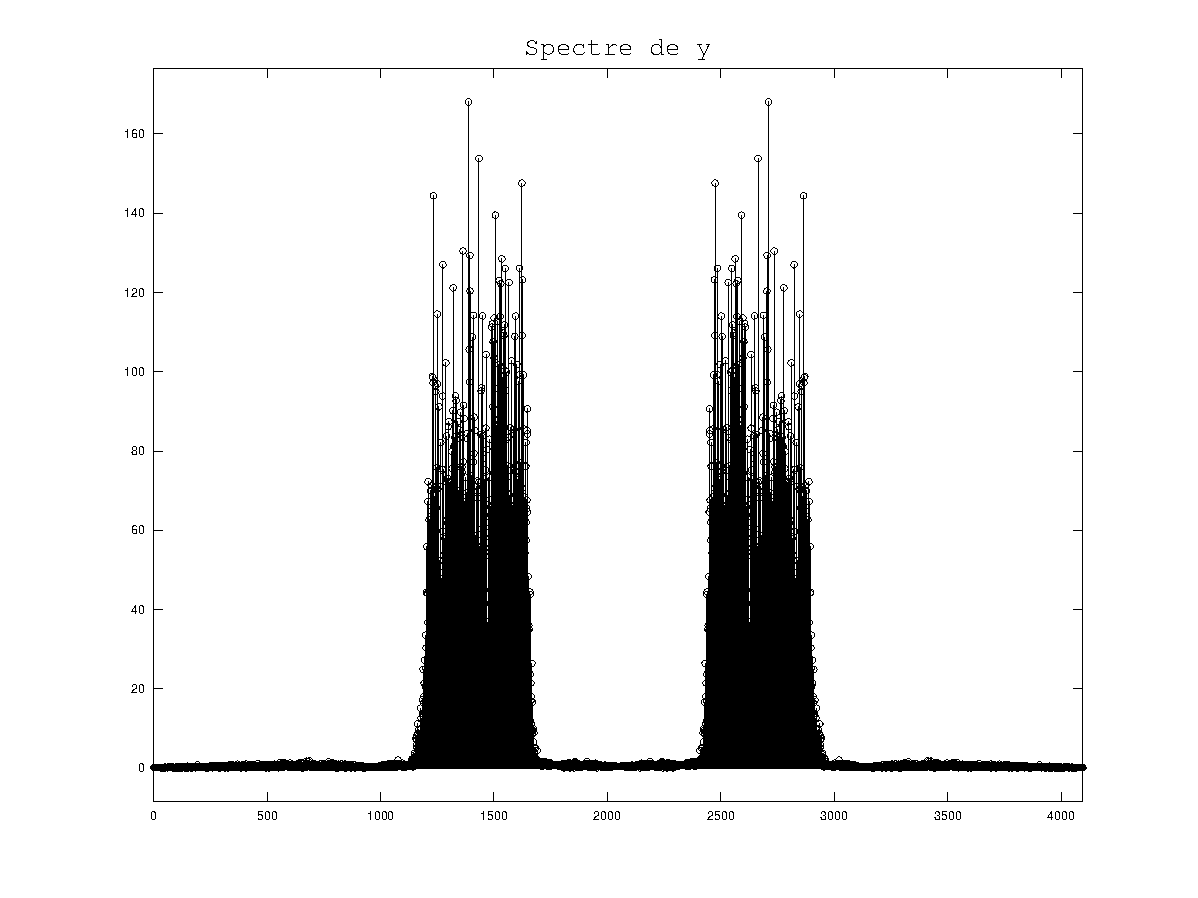
\includegraphics[width=9cm]{resEx6/fig_4.pdf}
\caption{Spectre de y}
\end{figure}


Les caractéristiques du signal x:\\
\begin{itemize}
\item Moyenne : 0.02
\item Ecart type : 1.01
\item Variance : 1.02
\end{itemize}


\begin{figure}[H]
\centering
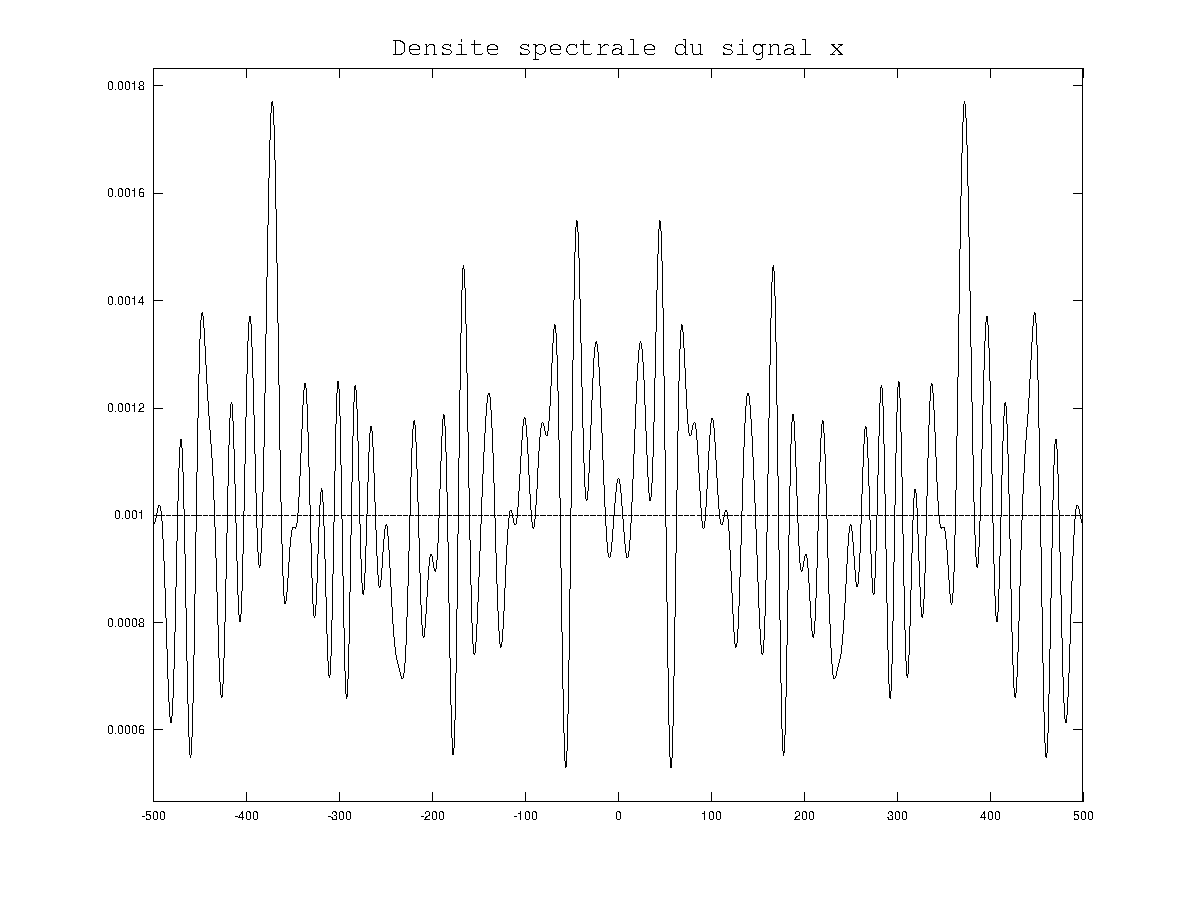
\includegraphics[width=9cm]{resEx6/fig_5.pdf}
\caption{Densite spectrale du signal x}
\end{figure}


\begin{figure}[H]
\centering
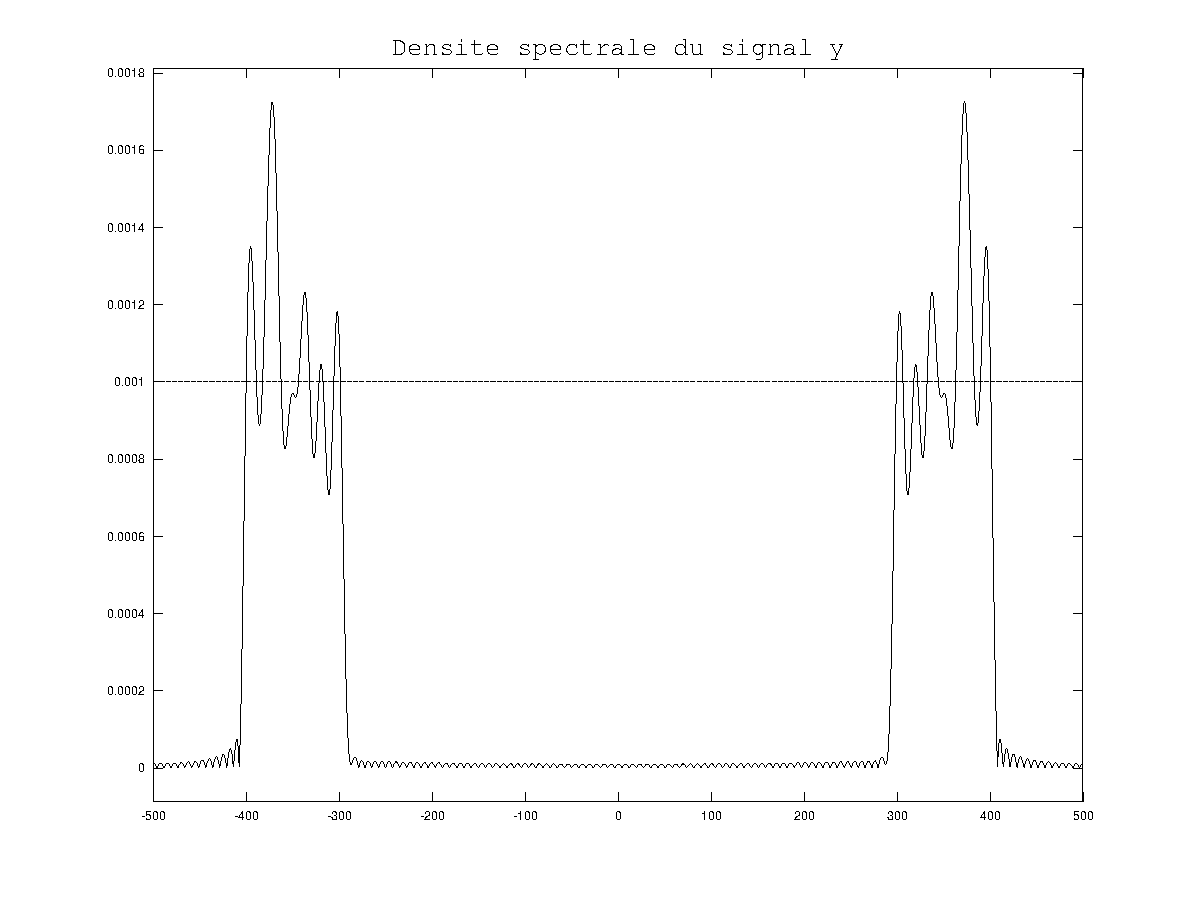
\includegraphics[width=9cm]{resEx6/fig_6.pdf}
\caption{Densite spectrale du signal y}
\end{figure}



Nous déduisons l’allure de la fonction de transfert harmonique du filtre grâce à la racine carré de la densité spectral en sortie / densité spectrale en entrée.

\begin{figure}[H]
\centering
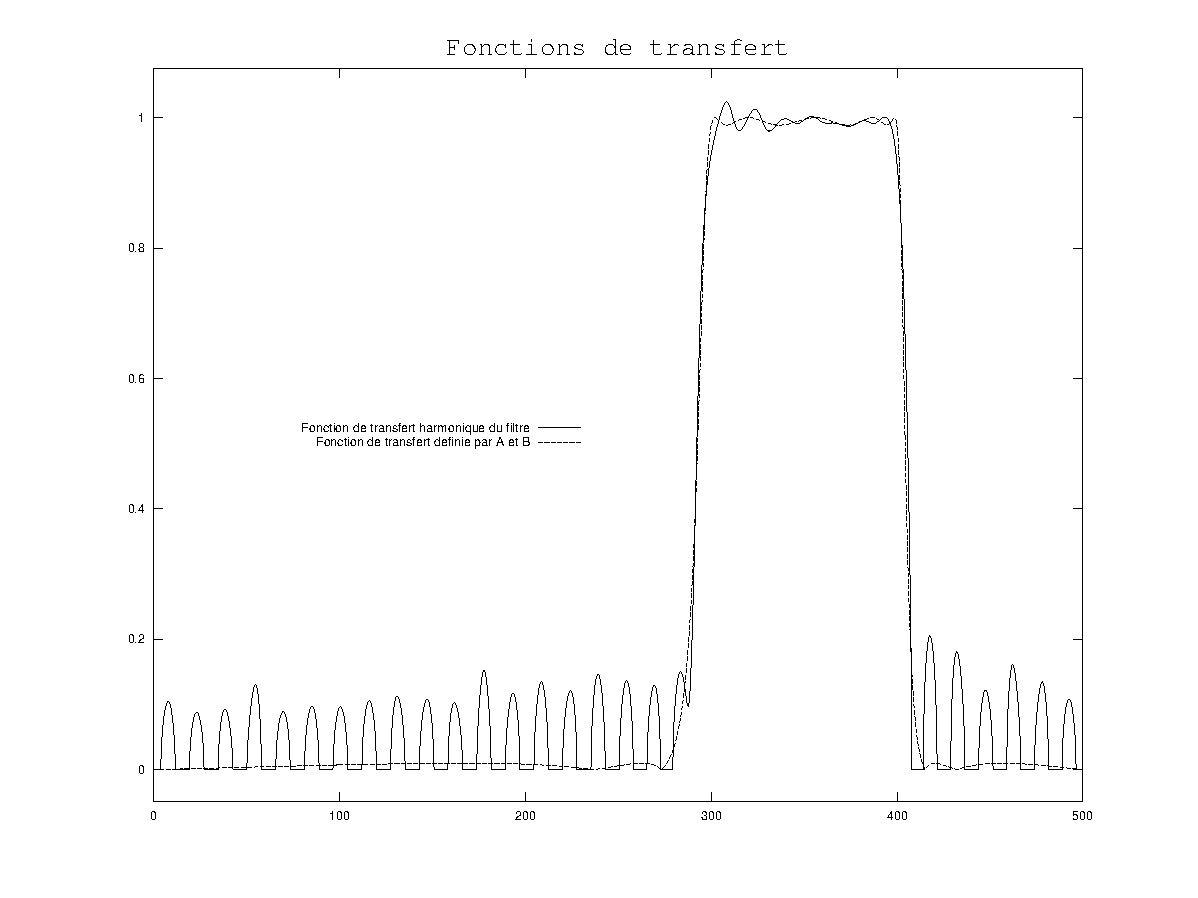
\includegraphics[width=9cm]{resEx6/fig_7.pdf}
\caption{Comparaison des Fonctions de transfert.}
\end{figure}

